%\documentclass[12pt]{article}
\documentclass[english]{sobraep}

\usepackage[utf8]{inputenc}
\usepackage[table]{xcolor}
\usepackage{geometry}
\geometry{a4paper, portrait, margin=2cm, top=2cm, bottom=2cm}
\usepackage{graphicx}
\usepackage{gensymb}
\usepackage{fancyvrb}
\usepackage{breqn}
\usepackage{times}
\usepackage{float}
\usepackage{svg}
\usepackage{tabularx}
\usepackage{lscape}
\usepackage{pdflscape}
\usepackage{biblatex}
\usepackage{amsmath}
\usepackage{blindtext}
\usepackage{hyperref}
\usepackage{cuted}
\addbibresource{references.bib}% Syntax for version >= 1.2

\title{Review of Recent Advancements in RMIS Using dVRK\\(ROBOTICS M - TECHNICAL ESSAY)}



%\author{Ross J. Gardiner\\
%	\normalsize \textbf{Email}: 2190583g@student.gla.ac.uk\\
%	\normalsize \textbf{Matric. nr.}: 2190583g
%}


\begin{document}
\maketitle
\begin{tabular}{l|c}
 Author: & \textbf{Ross J. Gardiner}   \\
 Course Code: & \verb|ENG5326| \\
 Matric Nr: & \verb|2190583g| \\
 Online: & \url{www.github.com}   \\
\end{tabular}
%\begin{minipage}{0.4\linewidth}
%\begin{figure}[H]
%    \centering
%    
\includegraphics[width=\textwidth]{university.eps}
%\end{figure}
%\end{minipage}
%\hfill
%\begin{minipage}{0.4\linewidth}
%\begin{figure}[H]
%    \centering
%    
\includegraphics[width=0.4\textwidth]{./university.eps}
%\end{figure}
%\end{minipage}
%\hfill
    
%\begin{center}
%    \vspace{35pt}
%    {\huge\textbf{ Review of Recent RMIS \\
%    Publications Using dVRK\\ \vspace{5pt}}}
        
%    \vspace{0.5cm}
%            Robotics M - Technical Essay
            
    
        
%    \vspace{5cm}
%        Ross Gardiner - 2190583g
        
%    \vspace{0.5cm}
%        February 2022
        
        
        
    
%    \vfill
        
%    \vspace{0.5cm}
%    James Watt School Of Engineering\\
%    University of Glasgow\\
            
%\end{center}


\setcounter{page}{1}
\pagenumbering{roman}
\thispagestyle{plain}
\begin{center}
    
    \textbf{Abstract}
\end{center}
\textbf{Minimally invasive surgery (MIS) has been shown to reduce patient trauma and accelerate recovery. Problems arising from the complex interface required by MIS are addressed with robotically assisted surgery. The clear market leading device for robotically assisted surgery is the da Vinci system from Intuitive Surgical. Additional input from the research community has enabled development of the da Vinci Research Kit (dVRK) - a comprehensive platform used in a wide range of recent research papers. In this report, recent advancements for robotically-assisted MIS (RMIS) are explored. This includes novel tooling mechanisms which integrate with the dVRK and enable new types of surgical procedures. Further, a review is given on some automation strategies for subordinate surgical tasks. This work showcases the research enabled by the dVRK and contributes some ideas for future developments using the platform.}

\begin{center}
    \textbf{Acknowledgements}
\end{center}
Special thanks to Robotics M course conveners, \textbf{Dr. Euan MacGookin} and \textbf{Dr. Kevin Worral} for teaching background required for this review and providing suggestions for academic journal sources. 
\pagenumbering{arabic}
\section{Introduction}
In this section, relevant topics for this report are introduced with context given. The need for RMIS is described and the dVRK shown as a key contributor in the literature. Further, some information is given on report structure and remaining areas for the report introduced. 
%In recent decades, key advancements in RMIS have allowed for cheaper, more repeatable and less damaging MIS surgery. Robotics in surgery continues to set This report includes details some such advances in the field, this is achieved by observation of kinematic aspects, investigation of the human-machine interface for RMIS surgery and a look at applications for artificial intelligence (AI) algorithms in the field. In this introduction, some further  concepts are introduced and structure for the remainder of this report is given. 


\subsection{RMIS}
Traditional surgery typically involved large incisions in the body to enable good visibility for the surgeon and ease of access for intricate manoeuvres. These large incisions can be damaging for the patient causing internal damage and scar tissue. This creates complications in recovery with many patients never making full return to health \cite{Nezhat2021}. A recent advance, Minimally Invasive Surgery (MIS) reduces collateral damage~\cite{laparoscopic-vs-open, intro-rmis}. 

MIS, also known as keyhole surgery, allows procedures to be completed with a minimal amount of incision. Complex tools and cameras are inserted to access inner areas of the body via small cut openings or natural orifices. Compared with open surgery, MIS drastically reduces patient trauma, accelerating recovery; the introduction of MIS surgeries have led to lower hospitalisation costs and higher levels of patient comfort ~\cite{laparoscopic-vs-open,intro-rmis}. One limitation of MIS noted throughout the literature is the uncomfortable and complex rigid tool operation required to manoeuvre within the body, while the use of cameras and viewing displays worsens hand-eye coordination \cite{intro-rmis, force-sensing}. This is not ergonomic - reducing dexterity, precision and causing fatigue for surgeons performing numerous or lengthy operations.

Robotically-assisted MIS (RMIS) attempts to address these issues via augmentation. Enhancement of the surgeons interface is facilitated by translation of human input to control of robotic manipulators. Typically, RMIS systems have a surgeon console, designed for comfort and Feedback to the surgeon is provided via sensing with the surgical instruments, this is presented to the surgeon with a human interface which may include several sensory integrations (ie 3D renders visualisation, haptic feedback and ).  The RMIS console also allows the surgeon console to be designed for comfort rather than other benefits of RMIS include simulated inputs for ease of training prospective operators without  

Ongoing research in the RMIS field is enabling high levels of dexterity and unparalleled surgical precision while providing a comfortable, ergonomic interface for surgeons.  

\subsection{Da Vinci and dVRK}
RMIS has seen wide adoption throughout the healthcare domain. Many systems have been brought to market for a wide range of surgical robotic tasks. Examples include `MicroHand' from \citeauthor{microhand2} which has recently completed first human trials \cite{microhand2} while the RAVEN-ii robotic surgical system presents a platform for researchers with special emphasis on modifiable software; although the system does not currently operate within appropriate safety margins for human operations \cite{raven-ii}. Two more RMIS research platforms are MiroSurge and M7 Surgical Robot~\cite[Table 1]{other-rmis-machines}.

The most abundantly used is the da Vinci system, first established in 1999 \cite{ergonomics, 10-years-dvrk}. This system has seen commercial success with over 5 thousand machines in operation worldwide. To date, over 7 million surgical procedures have been performed with da Vinci~\cite{10-years-dvrk}; Da Vinci is ubiquitous in industry and a desirable target for research innovations.

There are some modifications required for da Vinci to be used as a research platform. Primarily, devices are required to be modified for additional data acquisition, component exchange, software tweaks and upgrades. To facilitate researchers needs, \citeauthor{dvrk} introduced the da Vinci Research Kit (dVRK)~\cite{dvrk}. The dVRK is open sourced software and hardware allowing a standardised platform for RMIS research. In their publication, \citeauthor{dvrk} discuss in detail the mechanical, algorithmic, electronic and sensing aspects of their work and provide access to the dVRK via GitHub channels\footnote{\url{https://github.com/jhu-dvrk} - Accessed March 4\textsuperscript{th} 2022}~\cite{dvrk}. The dVRK provides a standardised, modular platform representative of the most popular RMIS machine in industrial use. 

Da Vinci systems and the dVRK have aided in extensive contributions to robotic surgery literature; \citeauthor{10-years-dvrk} report more than 25 thousand articles published using the dVRK platform~\cite{10-years-dvrk} since 2010. As dVRK is judged the most relevant and mature surgical research platform, this report focuses on publications which make use of it.  


\subsection{Report Structure}
Introductory material has explained the use-case for both MIS and its robotisation, showcased the da Vinci system and highlighted the significance of the dVRK to robotic surgery literature. For the remainder of this report, a search through the literature has been performed - largely aided by the existing review from \citeauthor{10-years-dvrk}~\cite{10-years-dvrk}. Areas of interest established are novel tooling additions compatible with the dVRK and automation of subordinate tasks for RMIS. Literature for each is summarised and analysis performed establishing the significance of the work. Following this, a conclusion reports overall findings and helps outline possible future research in line with these themes. 

\section{Tooling Additions}\label{sec:mechanical}
Da Vinci machines have a wide range of instrument attachments; a catalogue of tools is available on Intuitive Surgical's website~\cite{da-vinci-catalogue}. 
The dVRK platform enables development of new tooling attachments which may be integrated with da Vinci systems throughout the design process. In this section, two novel tools found in the literature are introduced and analysed. 
\subsection{Literature}
The da Vinci system lacks a device for cutting bone material. This is used for some MIS procedures, namely craniotomy~\cite{Fernandez-de_Thomas2022-ih};  a small part of bone is removed to provide access to areas within the skull. \citeauthor{bone-cutter} present an ultrasonic bone cutting tool integrated into the dVRK system~\cite{bone-cutter} (2018). Ultrasound is selected as the cutting method as it lacerates bone much easier than other tissues in the body - this is particularly advantageous for physically constrictive MIS where an abrasive method may erroneously cut tissues during insertion/manipulation. Design of the system is aided with a finite element analysis model, which is shown to compute a very close resonant frequency for laceration to that recorded in testing. Through use of the dVRK, the system is integrated to the da Vinci software and coupled mechanically. Denavit–Hartenberg parameters for control of the cutting end affector are also given~\cite[Table 3]{bone-cutter}. 
%bone cutter

%Soft actuator
Work from \citeauthor{soft-manip} showcase a new manipulator design for increasing 
A well known challenge for MIS is the ability to manoeuvre around and particularly behind organs to reach important areas. This requires a high degree of dexterity not always enabled by tooling used. \citeauthor{soft-manip} showcase a new manipulator design for improving dexterity using soft robotics, which has the added advantage of minimising damage to surrounding tissue~\cite{soft-manip} (2018). Through use of the dVRK, a da Vinci device is equipped with a novel pneumatic soft manipulator design. An endoscopic camera is attached to it's endpoint. Again, focus is given to the software and hardware integration with the dVRK. Control of the camera is facilitated via a foot-pedal at the surgeon console. A usability test of the system is carried out, asking non-experts to align the endoscope view with a selection of targets. The study participants are judged to be balanced and results show the controls devised to be easily learnable by humans.  

%something else

%algorithm selection

\subsection{Analysis}
Significant software and hardware engineering effort has been expended in design of these new apparatus. Both solutions show novel tooling. However, in both cases it is judged that much more extensive evaluations are required before tools reach the market. Work by \citeauthor{bone-cutter} includes laceration evaluation on a plastic bone simulator styrene outside of any MIS cavity. Evaluation could be made more realistic by adding spatial constraints to investigate 


\section{Automation and Augmented Control}\label{sec:Automation}
In the recent decade, advancements in deep learning and AI have shown machines capable of learning autonomous completion of a while array of tasks. Naturally, this has been applied to the robotic surgery domain in a range of publications \cite{shitloads}. This is judged as to be highly fruitful in the future development of RMIS; this section deals with some advances in automation specific to the dVRK. 

%RMIS systems may be operated by a surgeon 
%Many advancements in the RMIS field are made in the general area of the human-machine interface. In this section advancements in ergonomics and perceptual capabilities are discussed. 
\subsection{Literature - I}
\citeauthor{needle-grasp} present an extensive study on automated systems for robotic suturing. In their publication a novel design account is given for an algorithm to compute optimal needle grasp kinematics~\cite{needle-grasp}. 

To describe these kinematics, frames of reference are established. Figure \ref{fig:needle-frames} shows an adapted illustration. 
\begin{figure}[H]
    \centering
    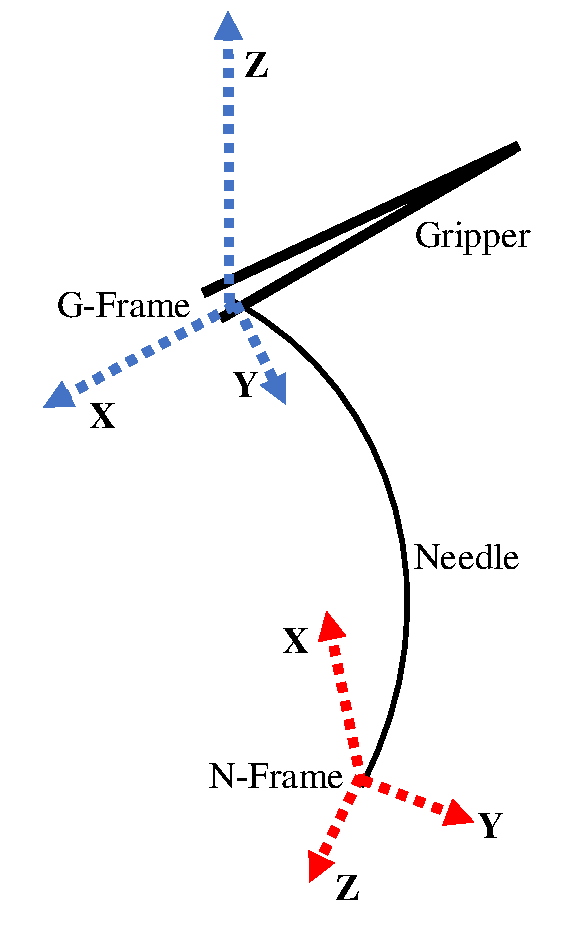
\includegraphics[scale=0.4]{figs/needle-frames.pdf}
    \caption{Gripper (G) and Needle (N) Frames of Reference (adapted from \cite[Figure 2(a)]{needle-grasp}). The G-Frame orients its origin at the tip of the gripper with Z-axis perpendicular to the gripper jaws; X-axis points parallel to the gripper, outwards. The N-Frame orients its origin at the needle tip, in this application needles are curved into a circular shape. The X-axis points towards the centre of needle curvature; Z-axis points tangent to the needle curvature, outwards.}
    \label{fig:needle-frames}
\end{figure}

With reference frames defined, four degrees of freedom are given for needle grasp. $\omega_{1}$ is rotation around the G-Frame Z-axis, $\omega_{2}$ is rotation around the G-Frame Y-axis, $\omega_{3}$ is rotation around an axis in the needle plane perpendicular with the X-axis in the N-Frame. Finally, $\vartheta_{0}$ is the insertion translation for the gripping point selected along the negative X-axis in the G-Frame. Following notation from the paper, $\varphi_0$ is the distance in insertion translation while $\varphi_1$, $\varphi_2$, $\varphi_3$ are respective rotation angles for $\omega_{1}$, $\omega_{2}$ and $\omega_{3}$. 

Forward-kinematics are then derived as a 4x4 translation matrix from the G-Frame reference to the N-Frame, denoted $g_{GN}$ and described by Equations \ref{eqn:matrix} \ref{eqn:R} and \ref{eqn:P} (where $s_n$ denotes $\sin(\varphi_n)$ $c_n$ denotes $\cos(\varphi_n)$ and $r_n$ is the radius of needle curvature). Copied below.
\begin{equation}
    g_{GN}(\varphi) = 
      \begin{bmatrix}
      R(\varphi) & P(\varphi)\\
      0 & 1
      \end{bmatrix}
      \label{eqn:matrix}
\end{equation}
\begin{equation}
    R(\varphi) =  
    \begin{bmatrix}
    s_1 s_3 - c_1 c_3 s_2 & - c_1 c_2 & - c_3 s_1 - c_1 s_2 s_3 \\
    -c_1 s_3 - c_3 s_1 s_2 & - c_2 s_1 & c_1 c_3 - s_1 s_2 s_3 \\
    -c_2 c_3 & s_2 & -c_2 s_3
    \end{bmatrix}
    \label{eqn:R}
\end{equation}
\begin{equation}
    P(\varphi) = 
    \begin{bmatrix}
    r_n c_1 s_2 (c_3 - 1)-r_n s_1 s_3 - \varphi_0\\
    r_n c_1 s_3 + r_n s_1 s_2 (c_3 - 1)\\
    r_n c_2 (c_3 - 1)
    \end{bmatrix}
    \label{eqn:P}
\end{equation}

Needle grasp variants may be explored by changing parameters $\varphi_0$, $\varphi_1$, $\varphi_2$ and $\varphi_3$. As some configurations are invalid due to reach-ability, joint limits and/or link collision constraints, a feasibility algorithm is developed to assert invalid end-affector positions. Finally, a needle grasp selection algorithm is constructed~\cite[Algorithm 1]{needle-grasp}. This operates by taking a set input of potential needle grasps and for each grasp the feasibility over given needle suturing trajectory positions is computed. For needle grasps and trajectory positions deemed feasible, some performance metrics are computed for later comparison.

In experimentation, 3410 pre-set needle grasp positions are evaluated for two suturing trajectories (described as ``needle insertion'' and ``needle extraction''). Findings show that 7.1\% of grasps are feasible for needle insertion with 30.1\% feasible for extraction. Finally, an optimal grasping pose is given which scores best on performance metrics is given for both trajectories. 

\subsection{Analysis - I}
This work details processes which may discount or otherwise compare needle grasp poses for the suturing task. However, for full automation of suturing the question remains as to how these initial pose candidates are generated. The authors mention that execution time for their algorithm is in the order of minutes for the 3410 poses used on a reasonably high end desktop machine. In a real world scenario the needle paths and kinematics would not be known before a surgery has begun - they would have to be computed ad-hoc. It is judged that minutes of processing time is too lengthy to expend during a surgical procedure. Thus, in its current form this is judged not usable in theatre. While the authors suggest that this may be remedied by implementing the algorithm in faster code, an alternative could be to use this algorithm as a method for generating examples of suitable grip poses given parameters dictating the environment. These data could be used for supervised deep learning to train a machine capable of guessing an optimal needle grasp for any given scenario.   
\subsection{Literature - II}


%In addition, automation of such tasks is thought to give rise to a new method for training robot operators. Work by 

\section{Conclusions}
This essay has investigated software and hardware innovations in RMIS looking specifically at the dVRK platform. For the tooling innovations discussed, it is judged that further evaluation work will better illustrate performance of both devices. For the automation methods, a suggestion is given that the gripper pose selection algorithm could be used as a data labelling mechanism for training a more general AI solution. In general, the utility of the dVRK is complemented throughout as an enabler of the research discussed. 

\printbibliography

\end{document}